\section{Matching}
\label{sec:match}
Matching foretages i to trin: Først bregnes den Euklidiske afstand ved ligning \eqref{euc}:
\begin{equation}
\sqrt{\sum\limits_{i=1}^n(F_i-F'_i)^2}
\label{euc}
\end{equation}
Givet to sæt af punkter $\bold{A}, \bold{A}'$, hver bestående af $(F, p)$, udregnes der for hver feature i $\bold{A}$, afstandene til features i $\bold{A}'$. Den feature i $\bold{A}'$ har den mindste euklidiske afstand, udvælges og der dannes par af punkter, der tilføjes til et midlertidigt sæt, af korrespondancer. Når alle inputs er blevet evalueret, sorteres de efter afstand, med korrespondancer af korteste afstand først. Hvis $|\bold{A}| > |\bold{A}'|$, er det garanteret, at mindst ét element(og muligvis flere) fra $\bold{A}'$, har flere matches, fra $\bold{A}$. Dette er ikke hensigtsmæssigt, da det antyder, at minimum ét af korrespondancerne er forkerte. Der er derfor anvendt en metode, til at sortere dårlige korrespondancer fra.
\\
\\
En tilgang kunne være, udelukkende at kigge på de $m$ bedste matches. Jo højere $m$ er, jo flere forkerte korrespondancer vil udvælges. For at sortere forkerte korrespondancer fra, anvendes en statistisk udregning. Denne metode, fjerner korrespondancer, der har en euklidiske afstand, der er mindre end middelværdien, af de 10 bedste matches, multipliceret med 5, hvilket er en empirisk defineret konstant. Det resulterende sæt af punkters motion-vektor, skal nu udregnes: $MV = p_i - p'_i$. 
$MV$'s standard afvigelse $s$ beregnes nu i x og y retningen. For x kan dette skrives: 
\begin{equation}
s_x = \sqrt{ \sum \limits_{n=1}^N (x_i  - \mu)^2 }
\label{pis}
\end{equation}
Iterativt fjernes punkter, hvis afstanden fra middelværdispunktet, er større, end standardafvigelsesafstanden, her opskrevet som en indikatorfunktion, der determinere om en korrespondance korrekt:
\begin{equation}
\begin{split}
indikator = 
\begin{cases}
1,&hvis \sqrt{(x_i - \mu_x)^2 + (y_i - \mu_y)^2} < \sqrt{s_x^2 + s_y^2} \\
0,& ellers
\end{cases}
\end{split}
\label{indikator}
\end{equation}
Ovenstående bliver gentaget, indtil en grænseværdi for standardafvigelsen er nået. Processen er illustreret, i figur \ref{fig:tilmatching}. Her ses, hvordan hver iteration fjerner forkerte korrespondancer, og bevæger sig tættere på en klynge af punkter, der må formodes at være inliers.
\begin{figure}[H]
    \centering
    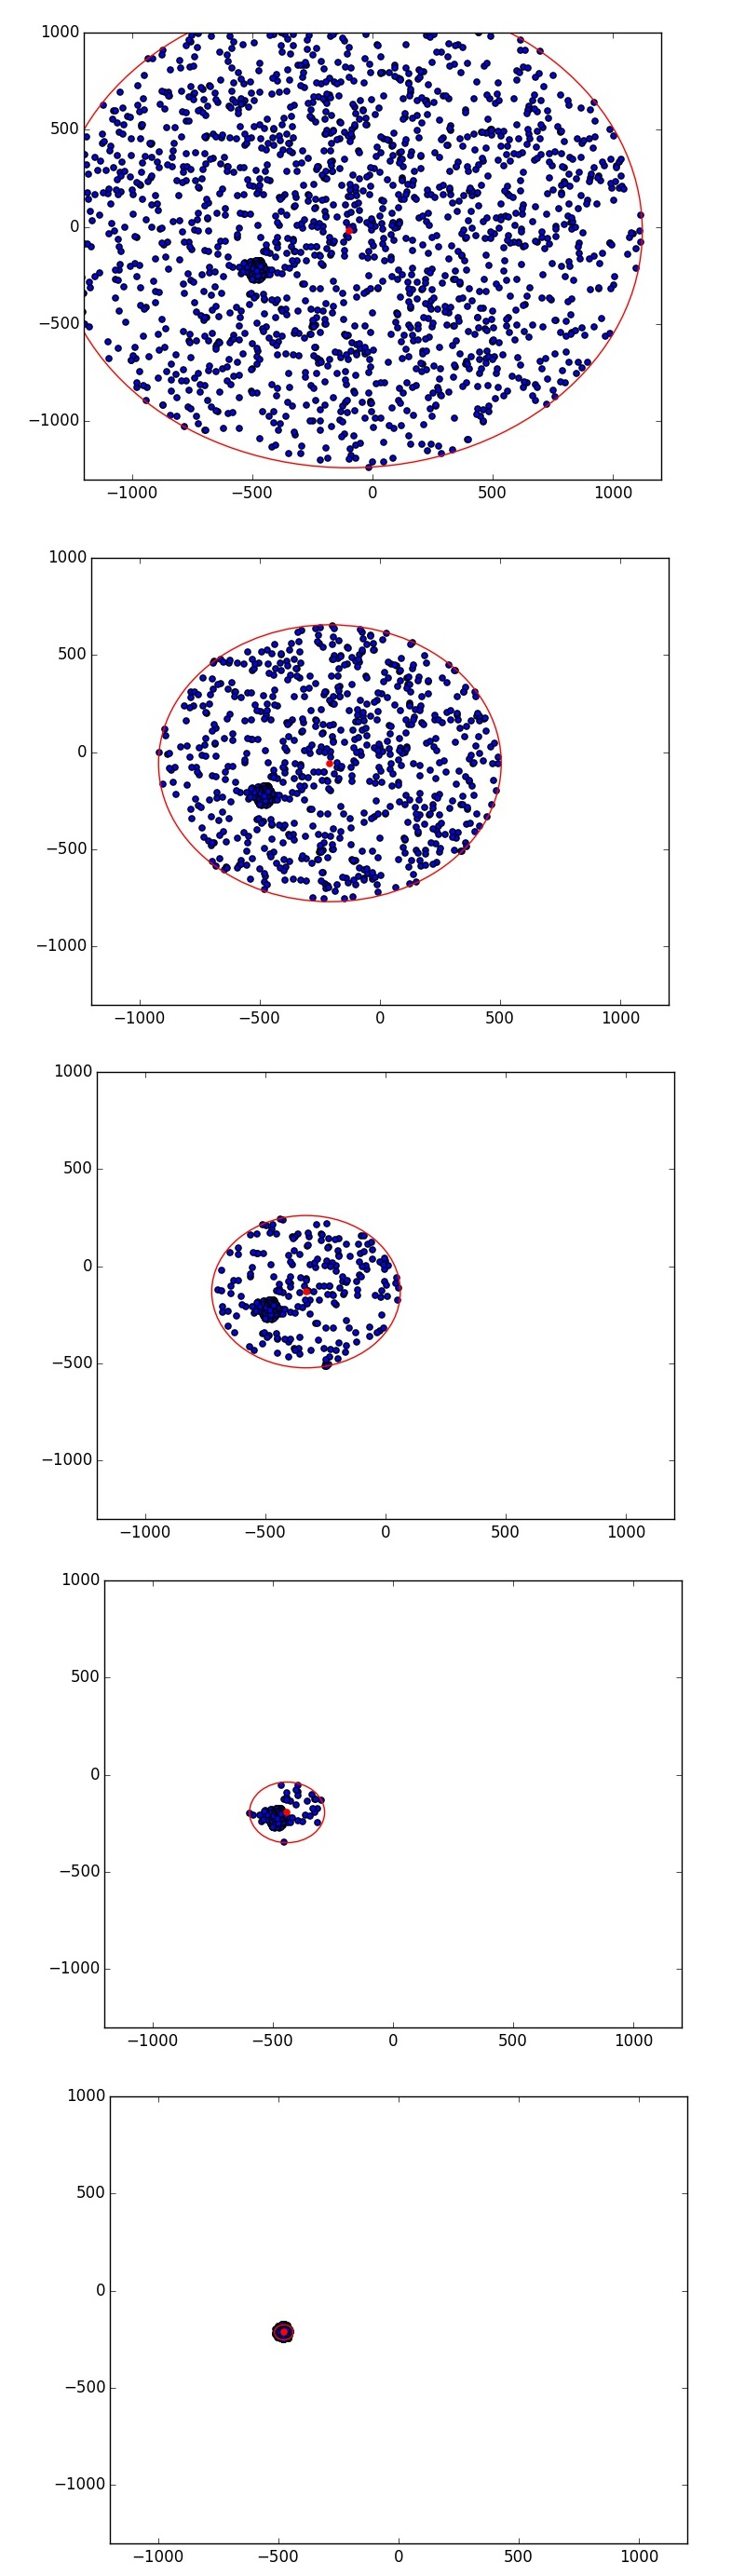
\includegraphics[width=0.99\textwidth]{fig/tilmatching.jpg}
     \vspace{-0.5em}
    \begin{center}    
       \caption{{\footnotesize \textit{Den røde cirkel medtager alle punkter, hvor ligning \eqref{indikator} gælder. Iterativt, bliver der fjernet punktet, indtil en grænseværdi er nået}}}
    \label{fig:tilmatching}
     \end{center}
     \vspace{-2.5em}
  \end{figure} \noindent

\subsection*{Algoritme}
\begin{tabbing}
Input\quad \= : \= Interessepunkter og tilegnede features: $\bold{A}$\\
Output \text{ } \> : \> Korrespondancer udledt til at være korrekte.
\end{tabbing}
\begin{enumerate}
\item{For hvert element i $\bold{A}$, udregnes den Euklidiske afstand som i ligning \eqref{euc}. Der bliver dannet par, af features i $\bold{A}'$, der har mindst euklidiske afstand til features i $\bold{A}$. Dette sæt kaldes $M$}
\item{$M$ sorteres, efter lavest euklidisk afstand.}
\item{Alle elementer af $M$, der har en afstand til hinanden, som er mindre end $5s$, fjernes fra $M$}
\item{Indikatorfunktionen fra ligning \eqref{indikator} bruges til at fjerne punkter, der er større end længden af standardafvigelsen}
\item{skridt 4 gentages, indtil ligning \eqref{pis} når en grænseværdi}
\end{enumerate}